\documentclass{scrreprt}
\usepackage{array}
\usepackage{graphicx}
\usepackage{listings}
\usepackage{underscore}
\usepackage[bookmarks=true]{hyperref}
\usepackage[utf8]{inputenc}
\usepackage{float}
\usepackage[french]{babel}
\hypersetup{
    bookmarks=false,    % show bookmarks bar
    pdftitle={rapport_Lambolez_Petit},    % title
    pdfauthor={Théodore Lambolez, Maximilien Petit},                     % author
    pdfsubject={TeX and LaTeX},                        % subject of the document
    pdfkeywords={TeX, LaTeX, graphics, images}, % list of keywords
    colorlinks=true,       % false: boxed links; true: colored links
    linkcolor=blue,       % color of internal links
    citecolor=black,       % color of links to bibliography
    filecolor=black,        % color of file links
    urlcolor=black,        % color of external links
    linktoc=page            % only page is linked
}
\def\myversion{1.0}
\date{}
%\title
\usepackage{hyperref}
\begin{document}
\begin{figure}
   \begin{minipage}[c]{.46\linewidth}
      
\includegraphics[scale=0.3]{telecom.png}
   \end{minipage} \hfill
   \begin{minipage}[c]{.46\linewidth}
      
\includegraphics[scale=1.9]{lorraine.jpg}
   \end{minipage}
\end{figure}
\begin{flushright}
    \rule{15cm}{5pt}
    \vskip1cm
\end{flushright}
\begin{center}
	\vspace{2.5cm}
	\fbox{
	\begin{minipage}{0.9\textwidth}
        	\Huge{
			\textbf{
			\begin{center}
				Rapport \\Gestion de Production \\Lasurex
				\vspace{0.5cm}
			\end{center}
			}
		}
	\end{minipage}
	}
\end{center}
\begin{flushright}
        \vspace{5cm}
	\huge{
        \textbf{
	Ecrit par \\
	\vspace{0,875cm}
	\href{mailto:theodore.lambolez@telecomnancy.eu}{Théodore Lambolez} \\
	\href{mailto:maximilien.petit@telecomnancy.eu}{Maximilien Petit}\\
	}
	}
        \vspace{0,5cm}
        \large{
	\textbf{
	\today\\
	}	
	}
\end{flushright}

\tableofcontents

\chapter{Première partie}

\paragraph{Contextes et objectifs généraux}
Cet exercice s'inscrit dans le cours de Gestion de Production afin de mettre en pratique les notions
vues en cours sur un ERP pédagogique :  Prélude. 

Tout au long de cet exercice, nous nous intéressons au cas de l'entreprise Lasurex qui fabrique deux
produits finis : les meubles lasurés (EML) et les meubles vernis (EMV). L'objectif de l'entreprise est 
de maximiser le taux de satisfaction client, de minimiser l'immobilisation des stocks et
le coût de réalisation de ces produits. Afin de réussir ces tâches, nous avons la possibilité de modifier le nombre de machines, l'ordonnancement ou encore le nombre d'heures de travail des employés. Cela nous a permis de mettre en application nos connaissances et d'analyser l'impact de l'utilisation des ressources dans le déroulement d'une entreprise.

Dans un premier temps, nous avons configuré l'ERP en le remplissant. Cette tâche nous a pris une séance de deux heures de TP à l'AIP. En effet, il a fallu prendre en main le logiciel Prelude et comprendre dans quel ordre remplir chacune des rubriques de l'onglet Données. Chaque donnée (postes de charges, articles, nomenclatures, gammes, prévisions, commandes, OAs, OFs) a des dépendances et nous avons dû les analyser afin de respecter celles-ci. Nous avions accès à des données dans la feuille PH1partiel.pdf distribuée en cours magistral. Au cours de celui-ci, nous l'avions complétée avec le professeur. Pour les articles, nous avons pris en compte le stock de sécurité, les besoins quotidiens et les lots multiples. Pour les nomenclatures, nous avons pris en compte les coefficients de lien. Chaque gamme est composé de phases où nous allons renseigner le temps de réglages et le temps unitaire de réalisation d'une tâche.

Dans un second temps, nous avons mis en place le premier ordonnancement dans le but de l'étudier. Cela nous a pris une séance de TP à l'AIP. Pour le mettre en place, nous avons procédé à une suite de méthodes : calcul des besoins nets, jalonnement, affermissement, ordonnancement. Puis, à chaque réalisation, vérifier la cohérence du résultat grâce aux programmes directeurs était obligatoire. Après plusieurs essais, nous n'arrivions pas à executer tous les OFs en temps voulu (impossible à programmer). Cela correspondait à la suite du TP, c'est à dire, modifier des données techniques afin de rendre le programme possible.


\chapter{Deuxième partie} 

\paragraph{Résultats de planification}

Au cours de notre première configuration, nous avons fait face à plusieurs erreurs dans la réalisation des OFs et OAs. Tout d'abord, les Ordres d'Achats correspondent aux moments où nous passons commandes afin d'avoir les produits M2 et M3 en temps et en heure pour la production. Ceux-ci sont configurés par nous-mêmes à l'avance ou suggérés par le logiciel. Cependant, certains n'ont jamais été programmés(impossible à placer) par les Ordres Fermes exécutés  ou jamais validés (impossible à supprimer). 

Le calcul des charges représente chaque OFs par semaine et donc la production réalisée en entreprise.
Elle permet de vérifier que tous les OFs ont été effectués et que le travail est régulier et équilibré
(contre exemple: une semaine légère puis une surchargée). De plus, il permet de vérifier que le jalonnement proposé est correcte afin de passer à la phase d'affermissement. Enfin, le calcul des charges indique, après analyse, les quantités de produits disponibles à la vente.



\chapter{Troisième partie}

\paragraph{Mise en oeuvre de solutions possibles}

Dans cette dernière partie, nous proposons des solutions afin de répondre à l'objectif principal : maximiser le taux de satisfaction client, minimiser l'immobilisation des stocks et
le coût de réalisation de ces produits. Nous commençons par un un ordonnancement à capacité finie au plus tard, pour charger les machines au maximum.


\begin{figure}[!h]
\centering
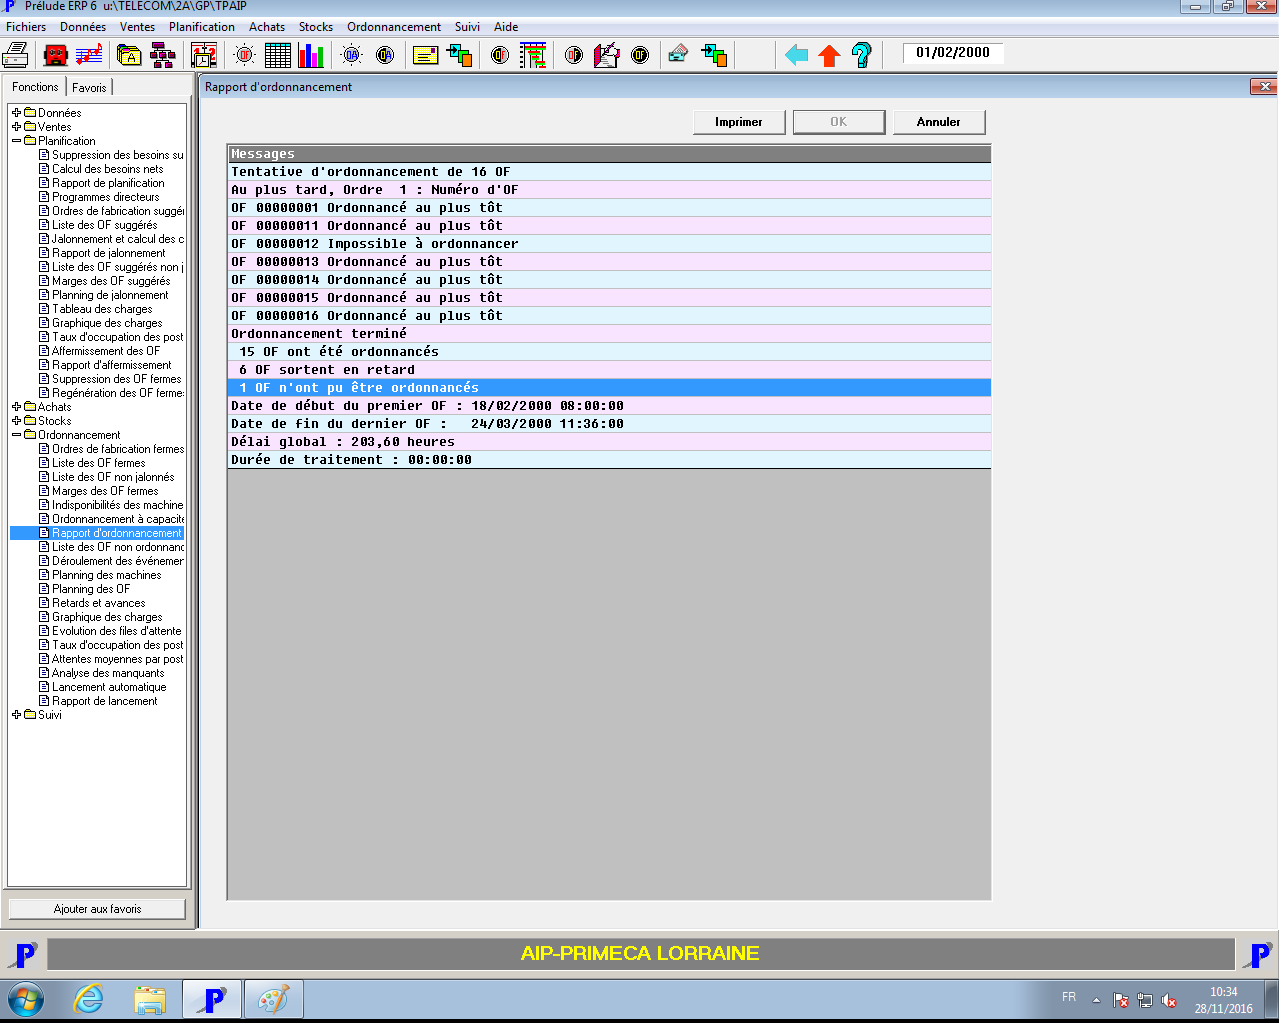
\includegraphics[width=10cm, height=5cm]{rapportAuPlusTard.png}
\caption{Résultat suite à l'ordonnancement à capacité finie avec option de gestion au plus tard}
\end{figure}

L'objectif ne peut pas être réalisé à temps, des ordres sont quand mêmes réalisés au plus tôt pour que les délais soit respectés. On peut en conclure que le délai est trop court pour réaliser tous les ordonnancements. Il faut donc trouver une autre solution. 

\newpage
Par exemple, on a essayé d’ajouter une machine de vernissage dans le but de réduire le taux de charge de chacune des machines. En effet, lorsqu’on regarde dans l’onglet permettant de consulter
les taux de charges de ces machines, on constatait que la machine de vernissage était surchargée.

\begin{figure}[!h]
\centering
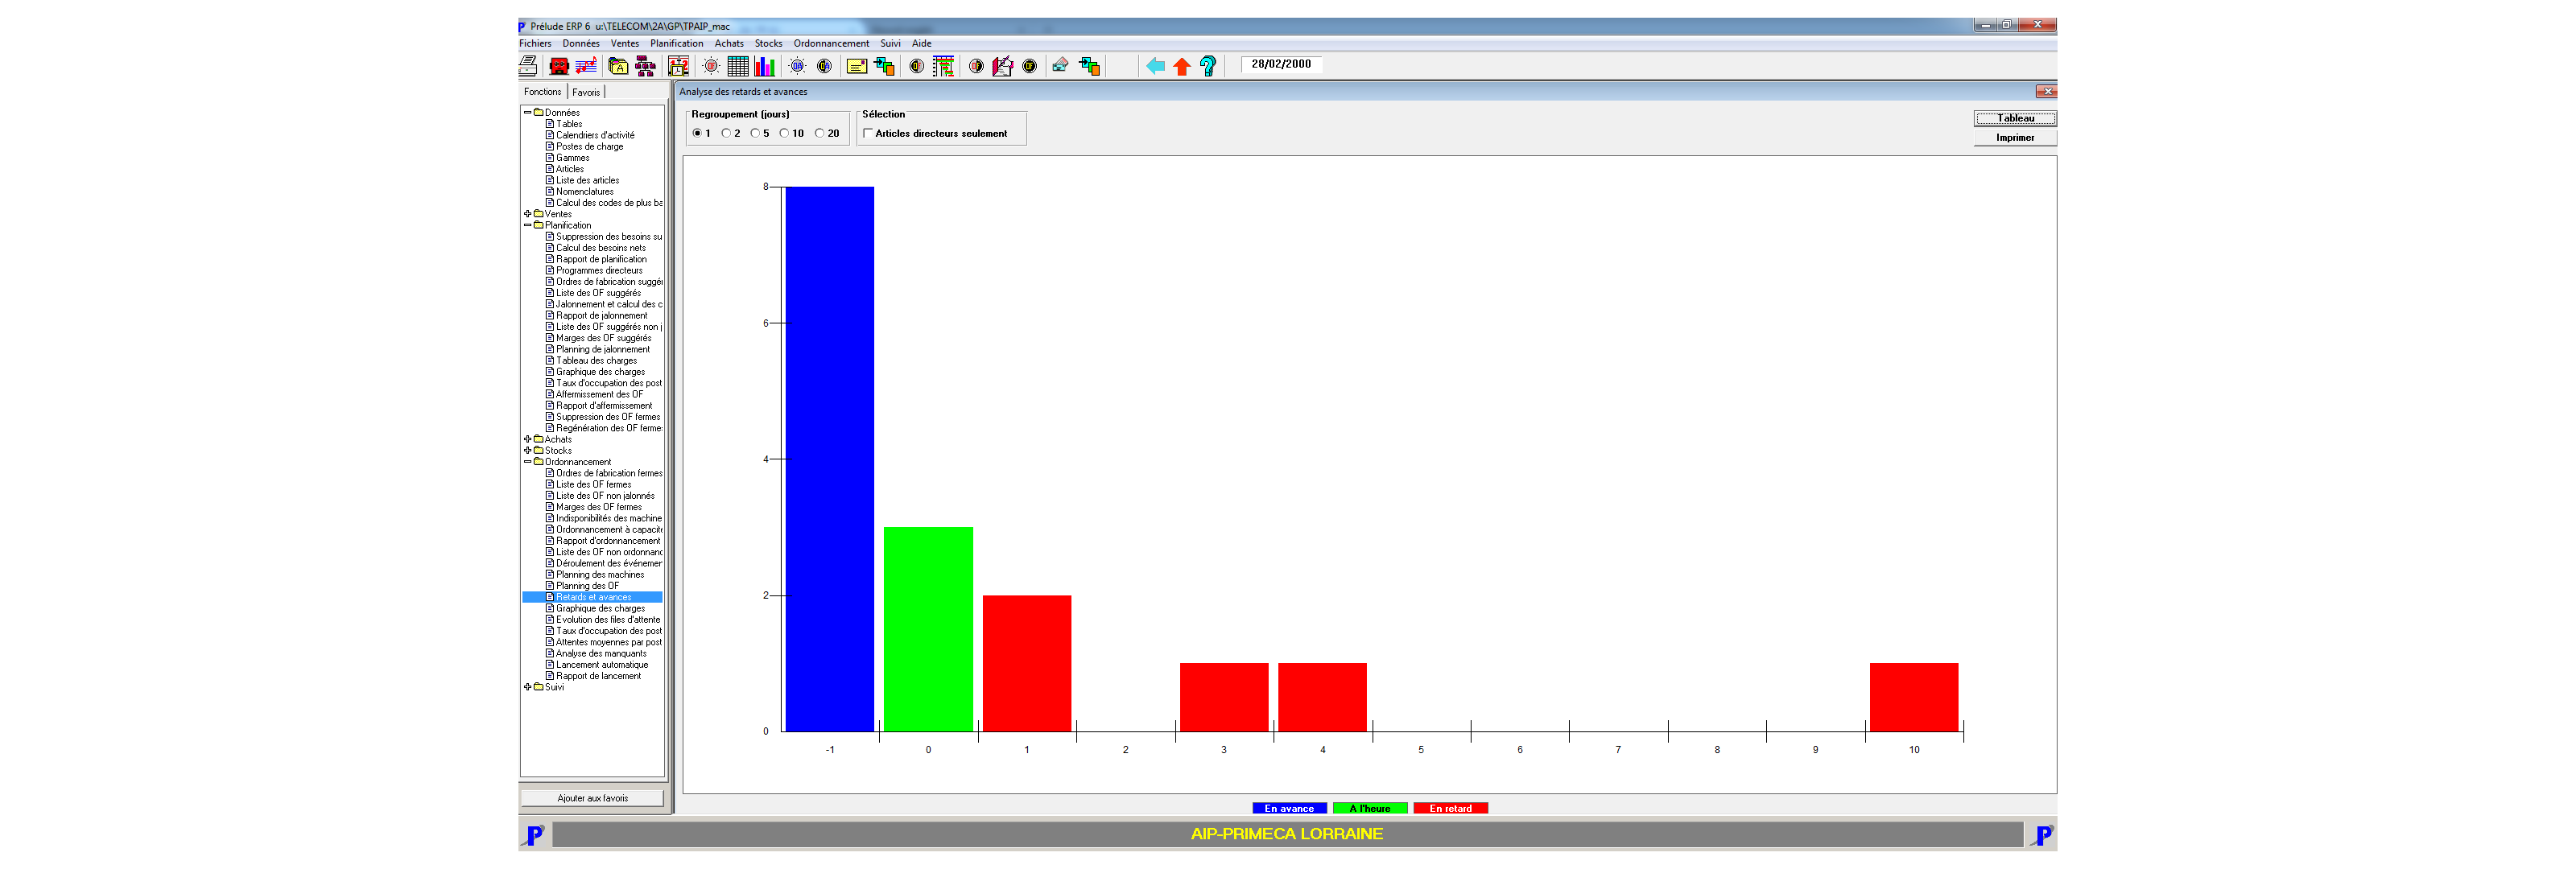
\includegraphics[width=10cm, height=5cm]{1vernisenplus.png}
\caption{Résultat suite à l'ordonnancement à capacité finie avec option de gestion au plus tard et une machine de vernissage supplémentaire}
\end{figure}


Tous les ordonnancements ont pu être placés mais il y a un retard trop important. On a rajouté une deuxième machine de vernissage. Le taux de charge n’a pas changé pour autant. On décide alors de s'orienter vers une autre modification. 

On a ajouté une équipe cette fois-ci : 

\begin{figure}[!h]
\centering
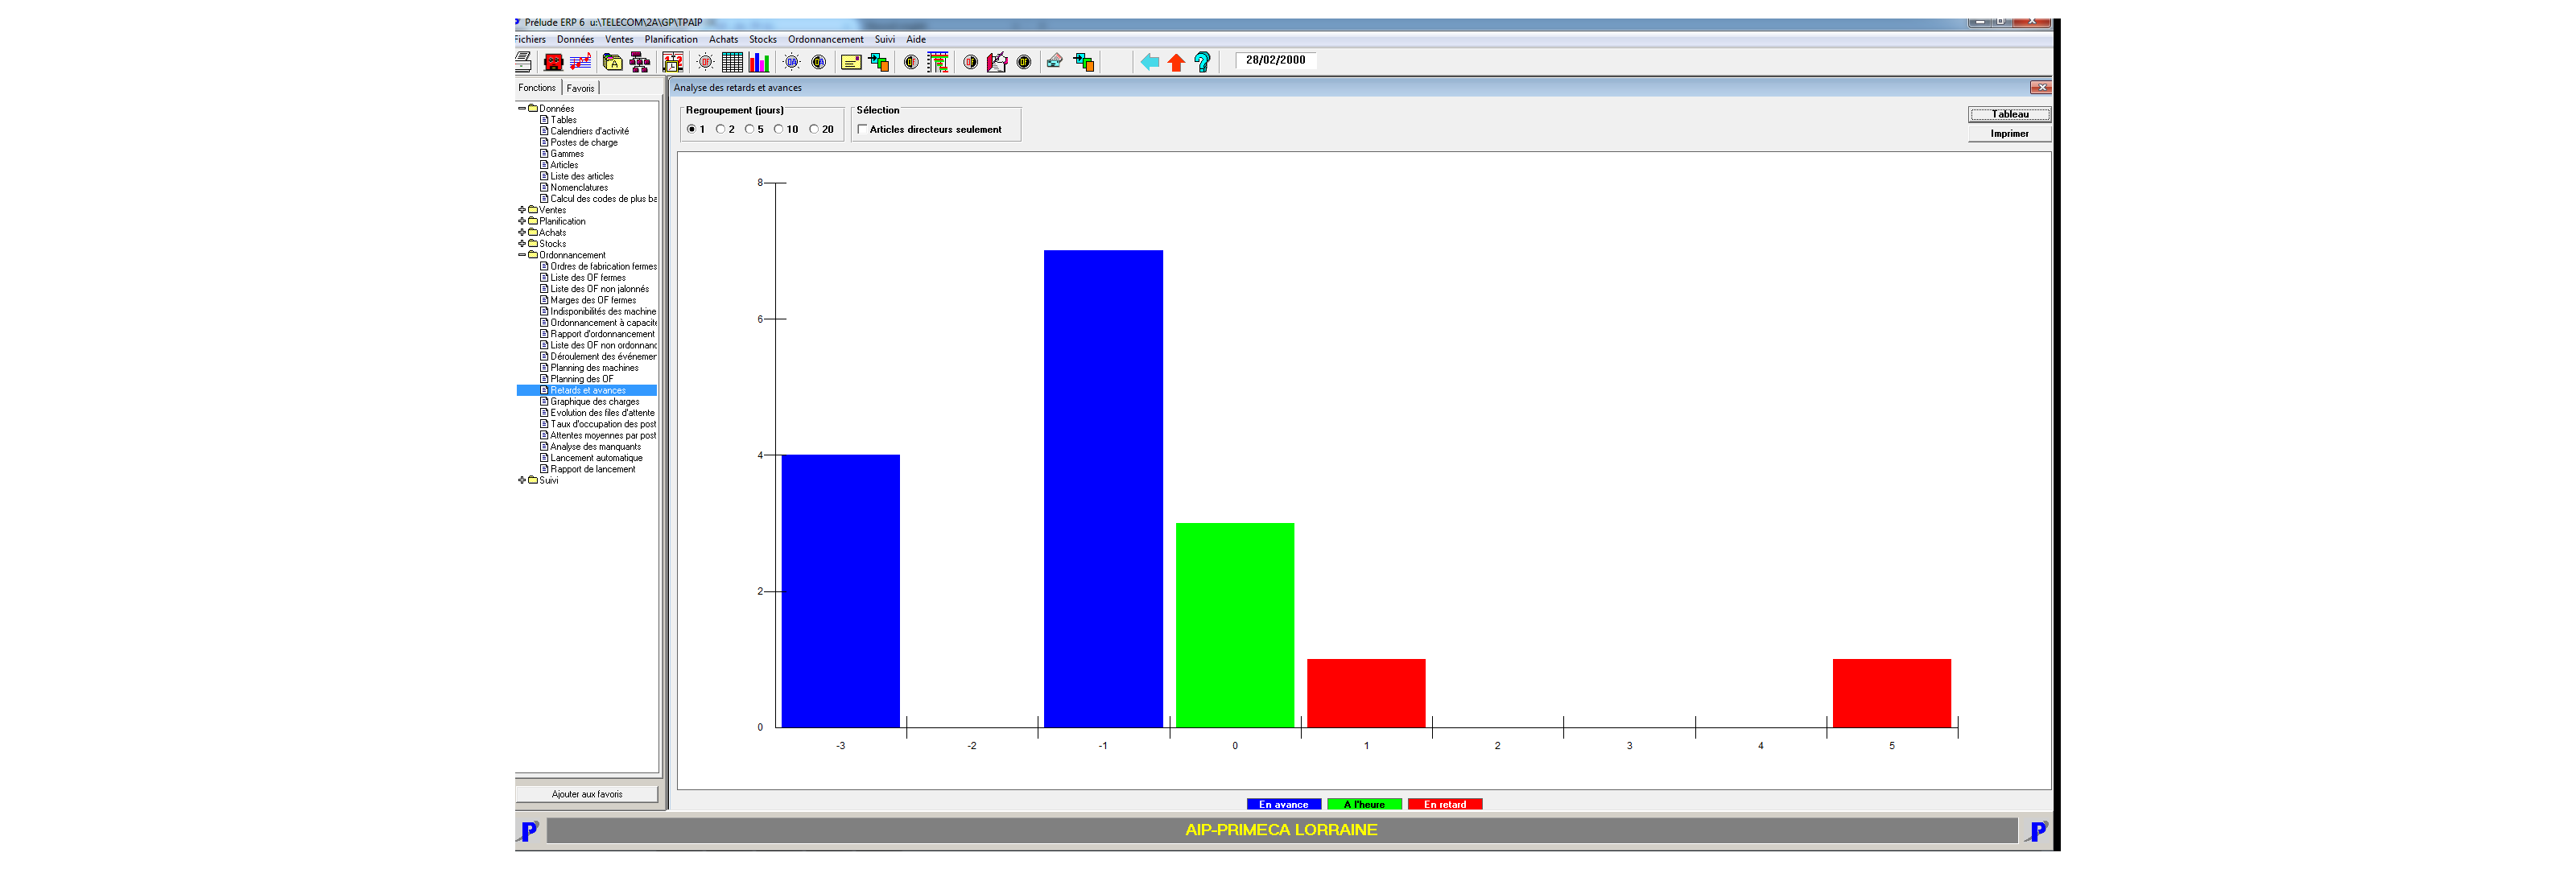
\includegraphics[width=10cm, height=5cm]{1equipeenplus.png}
\caption{Résultat suite à l'ordonnancement à capacité finie avec option de gestion au plus tard et une équipe supplémentaire}
\end{figure}


Toutes les OF ont été ordonnancés. Mais nous en avons trois en retard. Nous allons essayer de maximiser la satisfaction client en ajoutant une équipe de plus. La production sera donc active 24 heures sur 24.

\begin{figure}[!h]
\centering
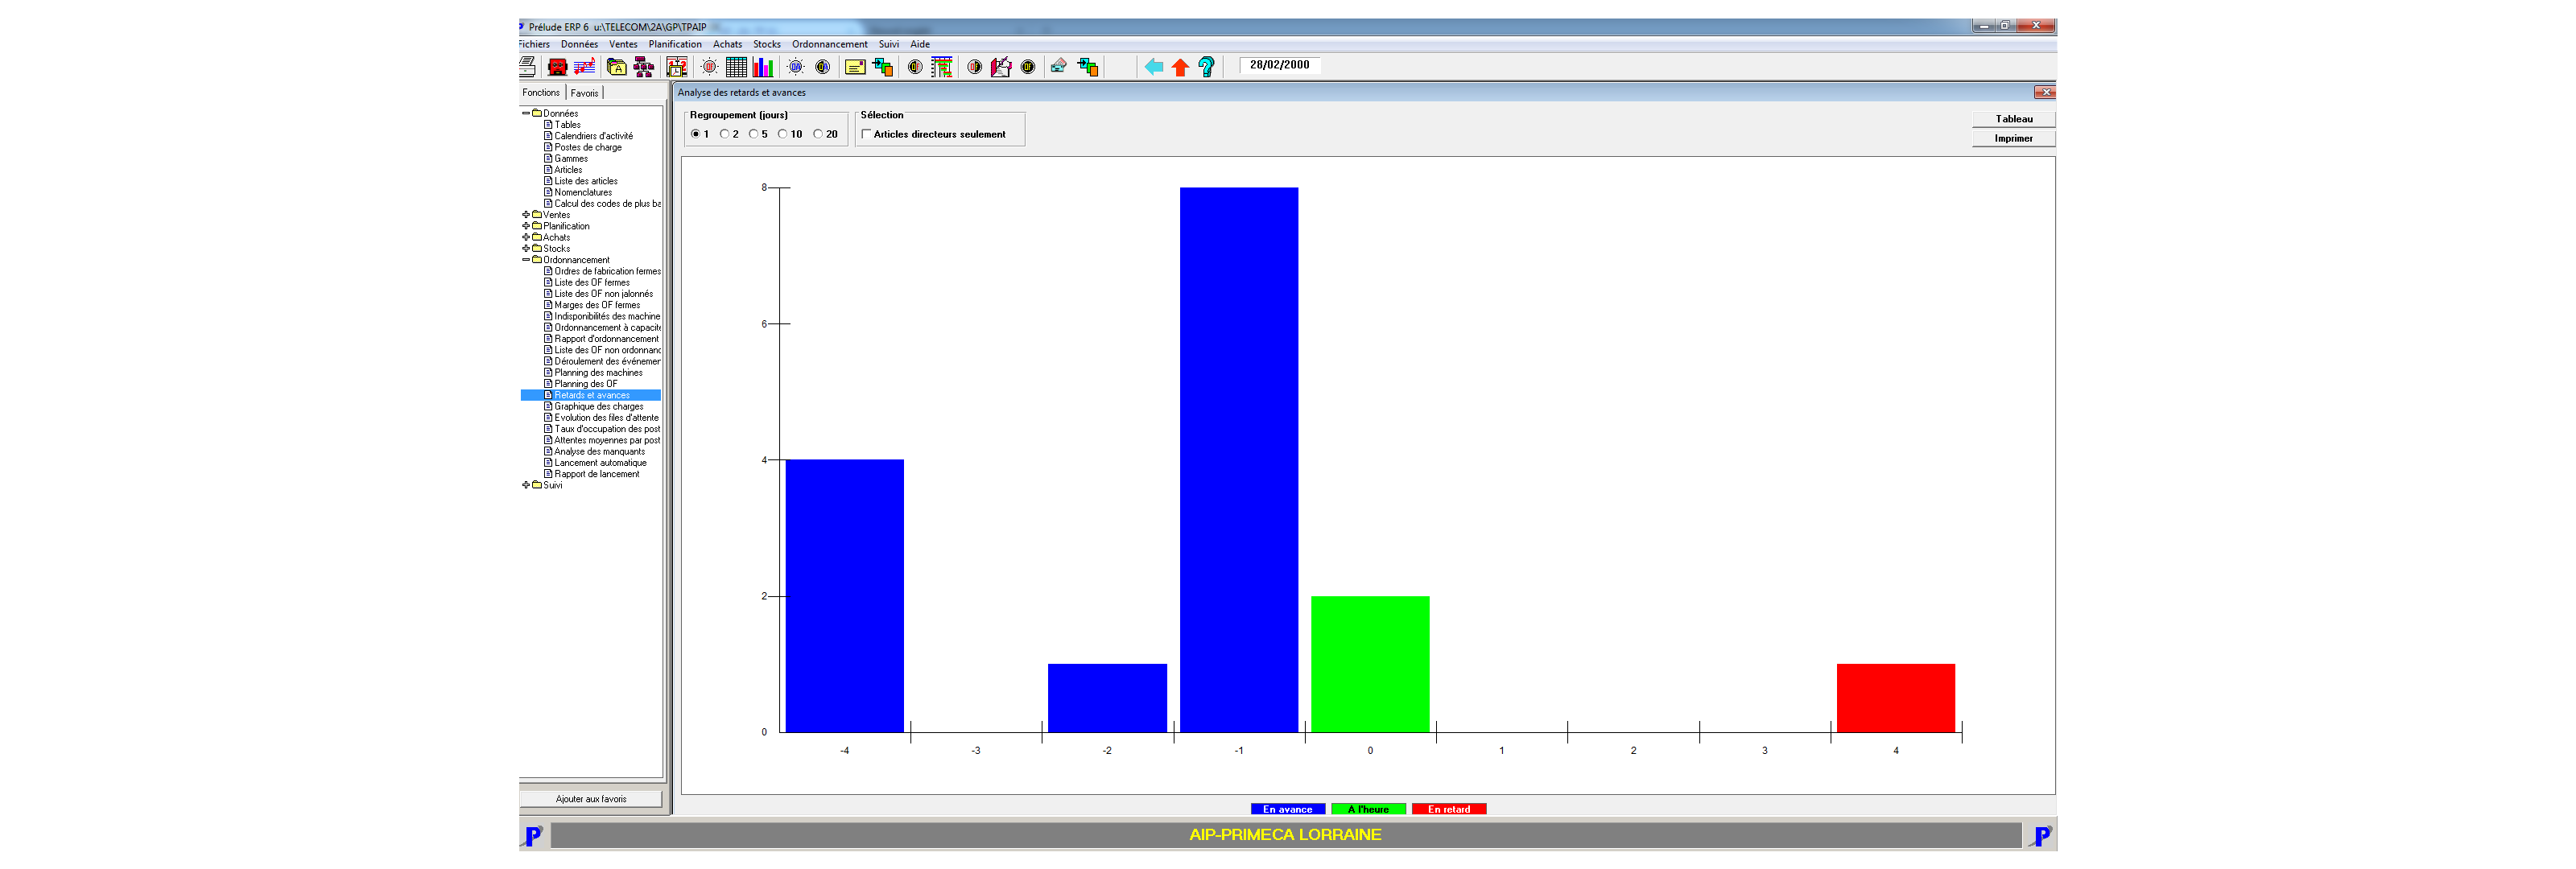
\includegraphics[width=10cm, height=5cm]{2equipeenplus.png}
\caption{Résultat suite à l'ordonnancement à capacité finie avec option de gestion au plus tard et deux équipes sumplémentaires}
\end{figure}

Avec cette configuration, nous n'avons plus qu'un OF en retard. Cependant, cette méthode génère des coûts supplémentaires en main d'oeuvre et en stocks.

Un autre ordonnancement possible est au plus tôt en décalant tous les OFs le plus tôt possible tout en respectant toutefois la date du 18 février. Cette organisation engendre 5 retards d'OFs mais moins de coûts de manière générale.

 \begin{figure}[!h]
\centering
\includegraphics[width=10cm, height=5cm]{RapportauPlusTotLancement.png}
\caption{Résultat suite à l'ordonnancement à capacité finie avec option de gestion au plus tôt}
\end{figure}

Pour conclure, l'achat de nouvelle(s) machine(s) permet la réalisation de tous les OFs au détriment d'un coût fixe important qui se répercutera sur le coût des produits finis.
De plus, on remarque qu'on a beaucoup d'OFs en avance ce qui implique qu'on aura des frais supplémentaires dûs au stocks.

L'emploi de plus de main d'oeuvre permet la réalisation de ce même critère (le taux de satisfaction client), cette fois-ci au détriment d'un coût supplémentaire régulier (le salaire des employés et le stock qui est très important avec deux équipes de plus). 

Enfin, si nous souhaitons minimiser les coûts supplémentaires tout en gardant un taux de satisfaction client acceptable, 
il est préférable de lancer les OFs plus tôt. L'anticipation est donc, ici, un moyen difficile à mettre en place mais moins coûteux. 

\end{document}